\documentclass[12pt]{article}

\usepackage[a4paper,margin=1in]{geometry}
\usepackage{booktabs}
\usepackage{listings}
\usepackage{xcolor}
\usepackage{amsmath}
\usepackage{graphicx}
\usepackage{float}
\usepackage{hyperref}

% -------------------------------------------------
% Code Style
% -------------------------------------------------

\definecolor{codegreen}{rgb}{0,0.6,0}
\definecolor{codegray}{rgb}{0.5,0.5,0.5}
\definecolor{codepurple}{rgb}{0.58,0,0.82}
\definecolor{backcolour}{rgb}{0.95,0.95,0.92}

\lstdefinestyle{pythonstyle}{
backgroundcolor=\color{backcolour},
commentstyle=\color{codegreen},
keywordstyle=\color{blue},
stringstyle=\color{codepurple},
numberstyle=\tiny\color{codegray},
basicstyle=\ttfamily\small,
numbers=left,
breaklines=true,
showstringspaces=false,
tabsize=4,
language=Python
}

\lstset{style=pythonstyle}

% -------------------------------------------------
% Report Details
% -------------------------------------------------

\title{
Deep Learning Laboratory\\
Assignment \#5
}

\author{
Siddharth Narayan Mishra\\
123CS0189
}

\date{\today}

\begin{document}

\maketitle

\tableofcontents

\newpage

%%%%%%%%%%%%%%%%%%%%%%%%%%%%%%%%%%%%%%%%%%%%%%%%%%%%%%%

\section*{How to read this report}
\addcontentsline{toc}{section}{How to read this report}

This report is written as a study guide rather than a bare lab writeup. Each
experiment starts with the plain idea, then the mathematics needed to follow the
code, then the code itself, then the numbers we actually got, and finally an
honest reading of what those numbers mean. Where a result looks disappointing,
the report explains why, because understanding why a method fails to help is
just as useful as seeing it succeed.

Both experiments were implemented from scratch using only \texttt{numpy},
\texttt{pandas} and \texttt{matplotlib}. There is no deep learning framework
involved: every forward pass, gradient, weight update, dropout mask and softmax
is written out by hand in \texttt{exp1.py} and \texttt{exp2.py}.

\paragraph{Settings shared by every model.}
Sigmoid activation in the hidden layers. Inputs standardized with a
\texttt{StandardScaler} that is fitted on the training split only (so the model
never peeks at test statistics). Weights initialized uniformly at random in
$[-0.5, 0.5]$, biases initialized to zero. Optimizer is stochastic gradient
descent with momentum, learning rate $0.001$, momentum $0.8$. Random seed $42$.
Thirty supervised epochs.

%%%%%%%%%%%%%%%%%%%%%%%%%%%%%%%%%%%%%%%%%%%%%%%%%%%%%%%

\part*{Experiment 1: Greedy Layer-wise Unsupervised Pre-training}
\addcontentsline{toc}{part}{Experiment 1: Greedy Layer-wise Pre-training}

\section{Objective}

\begin{itemize}
\item Build a deep classifier
      $X \rightarrow H_1 \rightarrow H_2 \rightarrow H_3 \rightarrow H_4
      \rightarrow Y$ with layer sizes $3\to3\to3\to3\to3\to1$ for the
      Social Network Ads dataset (predict whether a user purchased, from
      Gender, Age and EstimatedSalary).
\item Case 1: train this network directly with supervised learning and use it
      as the baseline.
\item Case 2: first pre-train each hidden layer one at a time, without using the
      labels, as an autoencoder; then stack the pre-trained layers, attach the
      output neuron, and fine-tune the whole thing with the labels.
\item Compare the two training curves and understand when this two-stage recipe
      is expected to help.
\end{itemize}

\section{Theory}

\subsection{The problem this method was invented to solve}

Around 2006, training deep networks made only of sigmoid layers was hard. The
reason is the \emph{vanishing gradient}. The derivative of the sigmoid
$\sigma(z) = 1/(1+e^{-z})$ is $\sigma(z)\,(1-\sigma(z))$, which is at most
$0.25$ and is much smaller than that whenever a neuron is even mildly saturated.
Backpropagation multiplies one such factor per layer. Through four hidden
layers the gradient reaching the first layer is scaled by roughly
$0.25^4 \approx 0.004$ in the best case and far less in practice. With a small
learning rate the early layers therefore barely move, and the network never
learns good low-level features.

Greedy layer-wise pre-training sidesteps this. Instead of trying to push a
gradient signal all the way down from the output, we teach each layer to do
something useful \emph{locally}, one layer at a time, and only then train the
full stack.

\subsection{Autoencoders in one paragraph}

An autoencoder is a network that is trained to copy its input to its output
through a narrow middle. It has an encoder that maps the input to a hidden
representation $h$, and a decoder that maps $h$ back to a reconstruction
$\hat{x}$. It is trained to minimise the reconstruction error, here the mean
squared error
\[
  \mathcal{L}_{\text{MSE}} = \frac{1}{N\,d}\sum_{i=1}^{N}\sum_{j=1}^{d}
  \bigl(\hat{x}_{ij} - x_{ij}\bigr)^2 .
\]
Because $h$ is forced to pass through a bottleneck, the encoder cannot just copy
the numbers across. It has to find a compact code that keeps whatever structure
is needed to rebuild the input. That code is exactly the kind of feature we
would like a hidden layer to compute. No labels are used, so this is
unsupervised learning.

\subsection{The greedy recipe used in Case 2}

\begin{enumerate}
\item \textbf{Stage 1.} Build an autoencoder
      $X \rightarrow H_1 \rightarrow \hat{X}$. Train it for 20 epochs on the
      training inputs. Keep the encoder weights $W_1$ (the part that produces
      $H_1$); throw the decoder away.
\item \textbf{Stage 2.} Freeze $W_1$. Push every training example through it to
      get the representation $H_1$. Build a new autoencoder
      $H_1 \rightarrow H_2 \rightarrow \hat{H_1}$ and train it for 20 epochs so
      that layer $H_2$ learns to reconstruct the output of layer $H_1$. Keep
      $W_2$.
\item \textbf{Stage 3 and Stage 4.} Repeat: $H_2 \rightarrow H_3$, then
      $H_3 \rightarrow H_4$. Every earlier layer stays frozen while the current
      one is trained.
\item \textbf{Assemble and fine-tune.} Stack $W_1, W_2, W_3, W_4$ into the deep
      network, add a fresh output neuron $H_4 \rightarrow Y$ with random
      weights, unfreeze everything, and train the whole network with the labels
      using binary cross-entropy for 30 epochs.
\end{enumerate}

The intuition is that fine-tuning now starts from a point where every layer
already computes something structured, instead of starting from random noise.
It is a smarter initialization, not a different model.

\subsection{The supervised loss}

The output neuron uses a sigmoid, so it produces a probability
$p \in (0,1)$ that the user purchased. Training minimises binary cross-entropy
\[
  \mathcal{L}_{\text{BCE}} = -\frac{1}{N}\sum_{i=1}^{N}
  \Bigl[\, y_i \log p_i + (1-y_i)\log(1-p_i) \,\Bigr] .
\]
This is small when the predicted probability is close to the true label and
grows without bound when the model is confidently wrong. Accuracy is reported
by thresholding $p$ at $0.5$.

\section{Algorithm}

\begin{enumerate}
\item Load the CSV. Encode Gender as Female $=0$, Male $=1$. Inputs are
      \texttt{[Gender, Age, EstimatedSalary]}, target is \texttt{Purchased}.
\item Make an 80:20 stratified train and test split (stratified means the
      purchased-to-not-purchased ratio is the same in both parts).
\item Fit \texttt{StandardScaler} on the training inputs, transform both splits.
\item \textbf{Case 1}: build the $3\to3\to3\to3\to3\to1$ network, train 30
      epochs with BCE, record train and test loss and accuracy each epoch.
\item \textbf{Case 2}: run the four pre-training stages above, assemble the
      network from the learned encoders, then fine-tune 30 epochs exactly as in
      Case 1.
\item Plot loss and accuracy curves for each case and a direct comparison.
\end{enumerate}

\section{Implementation}

A dense layer stores its weights, its bias, and one momentum buffer per
parameter. Forward keeps the pre-activation \texttt{z} and the activation
\texttt{a} so backward can use them.

\begin{lstlisting}
class Dense:
    def __init__(self, n_in, n_out, activation, rng):
        self.W = rng.uniform(-0.5, 0.5, size=(n_in, n_out))
        self.b = np.zeros(n_out)
        self.activation = activation
        self.vW = np.zeros_like(self.W)
        self.vb = np.zeros_like(self.b)

    def forward(self, x):
        self.x = x
        self.z = x @ self.W + self.b
        self.a = sigmoid(self.z) if self.activation == "sigmoid" else self.z
        return self.a

    def backward(self, da):
        dz = da * self.a * (1.0 - self.a) if self.activation == "sigmoid" else da
        self.dW = self.x.T @ dz
        self.db = dz.sum(axis=0)
        return dz @ self.W.T

    def step(self):                      # SGD with momentum
        self.vW = MOMENTUM * self.vW - LR * self.dW
        self.vb = MOMENTUM * self.vb - LR * self.db
        self.W += self.vW
        self.b += self.vb
\end{lstlisting}

One pre-training stage builds a small autoencoder (sigmoid encoder, linear
decoder so it can reconstruct real-valued standardized data), trains it, and
returns only the encoder:

\begin{lstlisting}
def pretrain_layer(representation, rng, epochs):
    dim = representation.shape[1]
    encoder = Dense(dim, 3, "sigmoid", rng)
    decoder = Dense(3, dim, "linear", rng)
    layers = [encoder, decoder]
    for _ in range(epochs):
        order = rng.permutation(len(representation))
        for start in range(0, len(representation), BATCH_SIZE):
            xb = representation[order[start:start + BATCH_SIZE]]
            out = net_forward(layers, xb)
            net_backward(layers, mse_grad(out, xb))   # target is the input
            net_step(layers)
    return encoder, losses
\end{lstlisting}

The Case 2 driver chains the stages, freezing earlier layers implicitly by
feeding the next stage the already-computed representation:

\begin{lstlisting}
representation = X_train.copy()
encoders = []
for stage in range(4):
    encoder, _ = pretrain_layer(representation, rng, PRETRAIN_EPOCHS)
    encoders.append(encoder)
    representation = encoder.forward(representation)   # move to next layer

layers = [copy_as_dense(enc) for enc in encoders]     # reuse learned weights
layers.append(Dense(3, 1, "sigmoid", rng))            # fresh output neuron
history = train_supervised(layers, X_train, y_train, X_test, y_test, 30, rng)
\end{lstlisting}

\section{Output}

\begin{figure}[H]
\centering
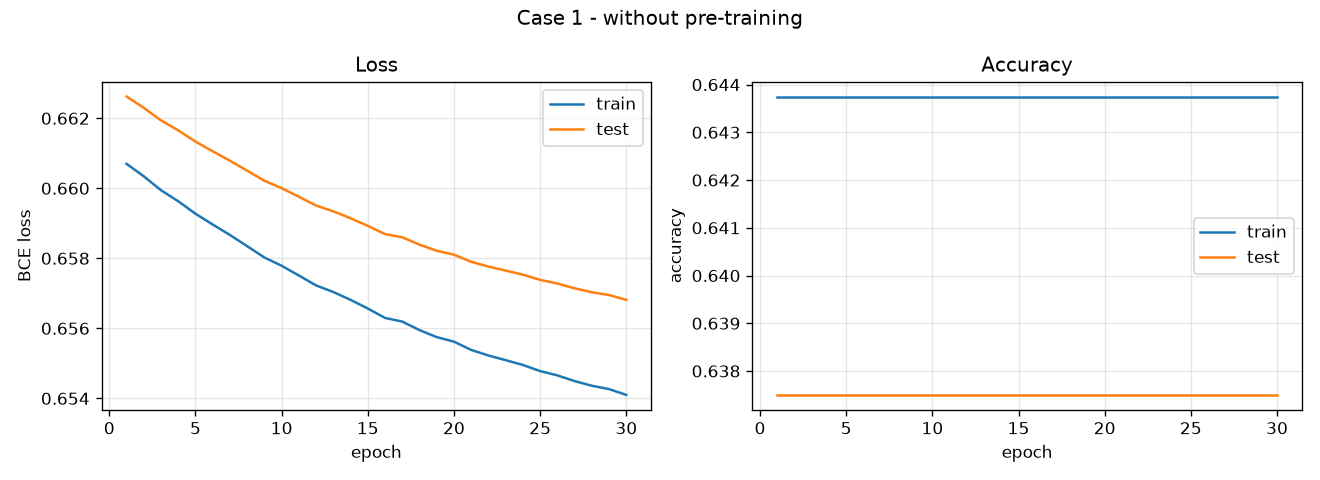
\includegraphics[width=0.95\linewidth]{case1.png}
\caption{Case 1, no pre-training. Loss falls slowly; accuracy is a flat line.}
\end{figure}

\begin{figure}[H]
\centering
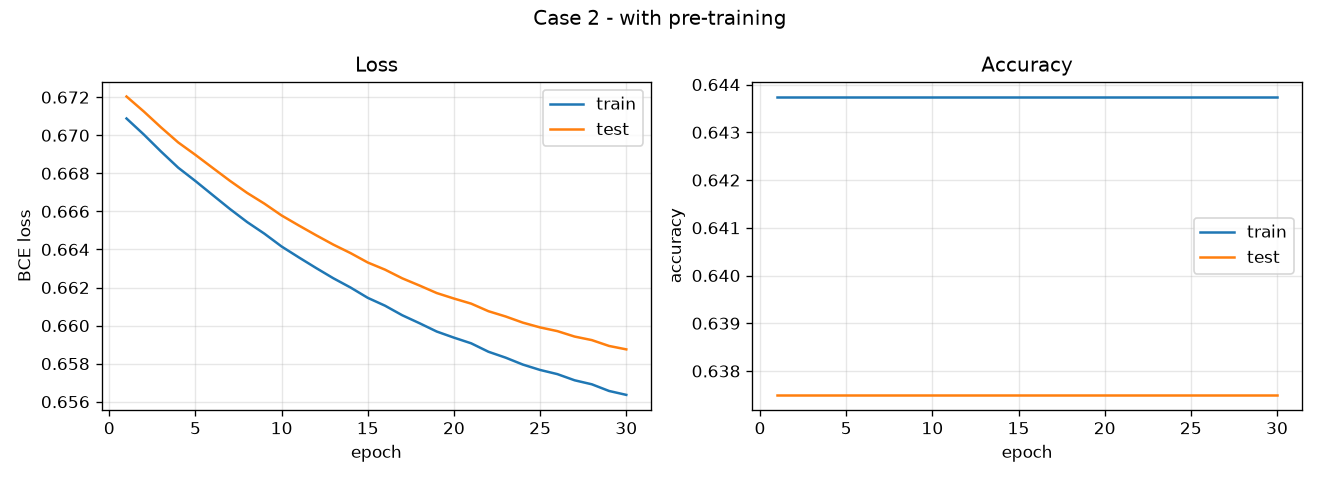
\includegraphics[width=0.95\linewidth]{case2.png}
\caption{Case 2, with pre-training. The picture is essentially the same as
Case 1.}
\end{figure}

\begin{figure}[H]
\centering
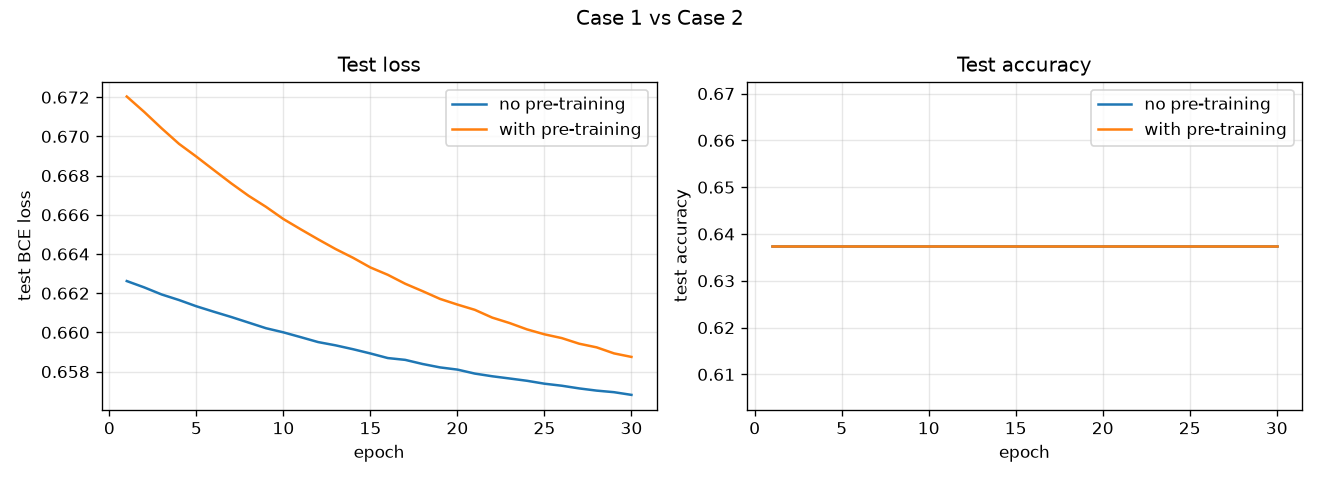
\includegraphics[width=0.95\linewidth]{case_comparison.png}
\caption{The two cases overlaid. The test-accuracy curves sit exactly on top of
each other.}
\end{figure}

\begin{table}[H]
\centering
\begin{tabular}{lcccc}
\toprule
 & train loss & test loss & train acc & test acc \\
\midrule
Case 1, no pre-training  & 0.6541 & 0.6568 & 0.6438 & 0.6375 \\
Case 2, with pre-training & 0.6564 & 0.6588 & 0.6438 & 0.6375 \\
\bottomrule
\end{tabular}
\caption{Final values at epoch 30.}
\end{table}

The reconstruction errors during pre-training were:

\begin{table}[H]
\centering
\begin{tabular}{lcc}
\toprule
stage & MSE at epoch 1 & MSE at epoch 20 \\
\midrule
1: $X \rightarrow H_1$   & 1.0077 & 0.9729 \\
2: $H_1 \rightarrow H_2$ & 0.2385 & 0.0451 \\
3: $H_2 \rightarrow H_3$ & 0.1124 & 0.0100 \\
4: $H_3 \rightarrow H_4$ & 0.1717 & 0.0134 \\
\bottomrule
\end{tabular}
\caption{Greedy pre-training, per-stage reconstruction MSE.}
\end{table}

\section{Observation}

\begin{itemize}
\item \textbf{Both models end up predicting the same single answer for
      everyone.} In the training set, $64.4\%$ of users did not purchase. A
      model that always says ``not purchased'' scores $63.8\%$ on the test set.
      Both Case 1 and Case 2 land on exactly that number and their accuracy
      curves are perfectly flat. The loss does drift down over the 30 epochs,
      which means the output neuron is nudging its bias to match the class
      ratio, but no model ever learns to separate buyers from non-buyers.
\item \textbf{Why nothing learns.} Four narrow sigmoid layers, a learning rate
      of $0.001$, and only 30 epochs together give the gradient no chance to
      reach the input side of the network. This is the vanishing-gradient
      situation described in the theory, reproduced on purpose by the fixed
      settings.
\item \textbf{Pre-training did work at its own job.} Stages 2, 3 and 4 drove the
      reconstruction error down by one to two orders of magnitude, so those
      layers genuinely learned to represent their inputs. Stage 1 barely moved,
      because squeezing standardized real-valued data through a single sigmoid
      of the same width and rebuilding it with a linear decoder, at this tiny
      learning rate, is close to hopeless in 20 epochs.
\item \textbf{Why pre-training still did not help the final accuracy.}
      Pre-training gives a better starting point, but fine-tuning then has to
      travel from that point to a good classifier using the same weak gradient
      signal. Here fine-tuning is so under-powered that it cannot exploit the
      head start. A better initialization is worthless if the optimiser that
      follows it cannot move.
\end{itemize}

\section{Conclusion}

Greedy layer-wise pre-training is an initialization trick for deep sigmoid
networks: train each layer as an autoencoder, stack the encoders, then
fine-tune with labels. In this experiment the pre-training phase measurably
learned to reconstruct the hidden representations, but the mandated training
budget (learning rate $0.001$, 30 epochs, four width-3 sigmoid layers) is far
too small for either the baseline or the pre-trained network to move off the
majority-class prediction, so the two cases finish with identical
$63.8\%$ test accuracy. The takeaway is conceptual: pre-training helps a deep
network find features it otherwise could not, but it cannot rescue a run whose
fine-tuning step is itself starved of gradient. With modern choices (ReLU
activations, a learning rate around $0.01$ to $0.1$, or a few hundred epochs)
both networks would learn the task, and the gap between them would shrink
further because good initialization matters most exactly when optimisation is
hard.

%%%%%%%%%%%%%%%%%%%%%%%%%%%%%%%%%%%%%%%%%%%%%%%%%%%%%%%

\newpage
\part*{Experiment 2: Regularization on Letter Recognition}
\addcontentsline{toc}{part}{Experiment 2: Regularization on Letter Recognition}

\section{Objective}

\begin{itemize}
\item Train a $16 \rightarrow 32 \rightarrow 16 \rightarrow 26$ classifier on the
      UCI Letter Recognition dataset (20{,}000 examples, 16 numeric features per
      example, one of 26 capital letters as the label).
\item Establish a baseline, then apply six well-known regularization or
      ensembling techniques, one per case.
\item For every case record the final test loss, test accuracy, and the
      $L_2$ norm of the trained weights, then compare how well each technique
      generalises and how large its weights end up.
\end{itemize}

\section{Theory}

\subsection{Generalisation, overfitting, underfitting}

We care about performance on data the model has never seen. Two things can go
wrong.

\begin{itemize}
\item \textbf{Overfitting}: the model memorises quirks of the training set. You
      see it as a widening gap where training accuracy keeps climbing while
      validation accuracy stalls or drops. Overfitting usually comes with large
      weights, because sharp decision boundaries need large numbers.
\item \textbf{Underfitting}: the model has not learned enough yet, from too
      little capacity, too few epochs, or too small a learning rate. You see it
      as training and validation curves that are close together and both still
      improving when time runs out.
\end{itemize}

Regularization is a family of techniques that fight overfitting by making the
model prefer simpler functions. The important caveat, which this experiment
demonstrates, is that regularization only helps when you were overfitting in
the first place. Applied to an underfitting model it just removes capacity the
model still needed.

\subsection{Softmax and sparse categorical cross-entropy}

With 26 classes the output layer has 26 neurons. Softmax turns their raw scores
$z_k$ into a probability distribution,
\[
  p_k = \frac{e^{z_k}}{\sum_{j=1}^{26} e^{z_j}},
  \qquad \sum_k p_k = 1 .
\]
The loss is the negative log probability the model assigned to the correct
class,
\[
  \mathcal{L} = -\frac{1}{N}\sum_{i=1}^{N} \log p_{i,\,y_i} .
\]
``Sparse'' just means the label is stored as an integer $0$ to $25$ rather than
as a length-26 one-hot vector; the maths is identical. A model that guessed
uniformly would score $\log 26 \approx 3.26$. The gradient of softmax combined
with this loss is the famously clean $p - \text{onehot}(y)$.

\subsection{The seven cases, each in a sentence or two}

\begin{description}
\item[Case 1, baseline.] The plain network. Everything else is measured
      against this.
\item[Case 2, $L_2$ regularization.] Add $\lambda \sum \|W\|^2$ to the loss
      (biases excluded), with $\lambda = 0.001$. The extra gradient term
      $2\lambda W$ pulls every weight slightly toward zero on each step, so the
      model keeps a weight large only if the data really pays for it. Result:
      smaller weights, smoother function.
\item[Case 3, input noise.] Add a small random perturbation to each training
      input every epoch (truncated Gaussian, standard deviation $0.1$, clipped
      to $[-1, 1]$). The model is forced to give stable answers in a little
      neighbourhood around each example, which is a mild form of data
      augmentation and is mathematically close to $L_2$.
\item[Case 4, label noise.] Randomly change $10\%$ of the training labels to a
      wrong class. This is not a technique you would choose; it tests how
      gracefully the model degrades when the training labels are dirty.
\item[Case 5, early stopping.] Train for at most 30 epochs but watch the
      validation loss. If it fails to improve by at least $0.001$ for $5$
      epochs in a row, stop and roll the weights back to the best epoch. The
      idea: the moment validation loss turns up is the moment the model starts
      overfitting, so freeze it there.
\item[Case 6, ensemble.] Train three networks with slightly different hidden
      sizes ($32\text{-}16$, $28\text{-}16$, $32\text{-}12$) independently,
      average their softmax probabilities,
      $P = (P_1 + P_2 + P_3)/3$, and predict the argmax of the average.
      Independent models make independent mistakes, so averaging cancels some
      of the error. This is the same reason the average of several noisy
      measurements is more reliable than any single one.
\item[Case 7, dropout.] During training only, randomly zero $50\%$ of the units
      after $H_1$ and $20\%$ after $H_2$, rescaling the survivors so the
      expected sum is unchanged. No unit can rely on any other specific unit
      being present, so the network learns redundant, robust features. At test
      time dropout is switched off and the full network is used.
\end{description}

\subsection{Why report the weight norm}

The $L_2$ norm of all weight matrices stacked together,
$\|W\|_2 = \sqrt{\sum_{\text{layers}} \sum_{ij} W_{ij}^2}$, is a simple proxy
for how ``aggressive'' the learned function is. Techniques that regularise by
shrinking the function (L2, dropout) should show a smaller norm than the
baseline; techniques that do not (input noise, early stopping here) should look
similar; an ensemble has a larger combined norm simply because it is three
models.

\section{Algorithm}

\begin{enumerate}
\item Load \texttt{letter-recognition.data}. Map the letter A to Z to integers
      $0$ to $25$. Features are the 16 integer columns.
\item Make a 60:20:20 stratified train, validation, test split.
\item Fit \texttt{StandardScaler} on the training inputs only, transform all
      three splits.
\item For each case, build the network, train with the case-specific
      modification for 30 epochs (fewer if early stopping fires), tracking
      training and validation loss and accuracy each epoch.
\item After training, evaluate on the held-out test split and record test loss,
      test accuracy and $\|W\|_2$.
\item Plot training and validation loss and accuracy against epoch for each
      case, and collect all seven results into one table.
\end{enumerate}

\section{Implementation}

The softmax-plus-cross-entropy gradient, written directly as $p - \text{onehot}$
and averaged over the batch:

\begin{lstlisting}
def scce_grad(probs, y):
    grad = probs.copy()
    grad[np.arange(len(y)), y] -= 1.0
    return grad / len(y)
\end{lstlisting}

$L_2$ regularization is one extra term added to the weight gradient inside the
optimiser step (note it never touches the bias):

\begin{lstlisting}
def step(self, l2):
    dW = self.dW + 2.0 * l2 * self.W if l2 else self.dW
    self.vW = MOMENTUM * self.vW - LR * dW
    self.vb = MOMENTUM * self.vb - LR * self.db
    self.W += self.vW
    self.b += self.vb
\end{lstlisting}

Dropout is applied between layers during the training forward pass and the same
mask is reused in backward. The division by \texttt{(1 - rate)} is the
rescaling that lets us leave the network untouched at test time:

\begin{lstlisting}
def forward_dropout(layers, x, dropout, rng):
    masks = {}
    for i, layer in enumerate(layers):
        x = layer.forward(x)
        if dropout and i in dropout:
            rate = dropout[i]
            mask = (rng.random(x.shape) >= rate) / (1.0 - rate)
            x = x * mask
            masks[i] = mask
    return x, masks
\end{lstlisting}

Input noise is resampled once per epoch and added to a shuffled copy of the
training inputs, leaving validation and test untouched:

\begin{lstlisting}
order = rng.permutation(n)
X_epoch, y_epoch = X_train[order], y_train[order]
if input_noise_sigma:
    X_epoch = X_epoch + truncated_normal(input_noise_sigma, X_epoch.shape,
                                         clip=1.0, rng=rng)
\end{lstlisting}

Early stopping keeps the best weights seen so far and counts epochs without
improvement:

\begin{lstlisting}
if es["best_loss"] - val_loss > ES_MIN_DELTA:
    es.update(best_loss=val_loss, best_epoch=epoch, wait=0,
              best_snapshot=snapshot(layers))
else:
    es["wait"] += 1
    if es["wait"] >= ES_PATIENCE:
        es["stop_epoch"] = epoch
        break
# after the loop: restore(layers, es["best_snapshot"])
\end{lstlisting}

The ensemble simply averages probabilities from the three trained models:

\begin{lstlisting}
p_test = np.mean([predict(m, X_test) for m in members], axis=0)
ensemble_acc = np.mean(np.argmax(p_test, axis=1) == y_test)
\end{lstlisting}

\section{Output}

\begin{table}[H]
\centering
\begin{tabular}{lccc}
\toprule
Case & Test loss & Test accuracy & $\|W\|_2$ \\
\midrule
1. Baseline                       & 2.3668 & 0.3788 & 15.84 \\
2. $L_2$, $\lambda = 0.001$       & 2.5123 & 0.3411 & 13.46 \\
3. Input noise, $\sigma = 0.1$    & 2.3707 & 0.3808 & 15.80 \\
4. Label noise, $10\%$            & 2.4345 & 0.3958 & 15.14 \\
5. Early stopping                 & 2.3668 & 0.3788 & 15.84 \\
6. Ensemble (average of 3)        & 2.4110 & \textbf{0.4540} & 26.30 \\
7. Dropout, $0.5 / 0.2$           & 2.7064 & 0.3073 & 12.85 \\
\bottomrule
\end{tabular}
\caption{All seven cases on the held-out test split. Uniform guessing would
give accuracy $1/26 \approx 0.038$ and loss $\approx 3.26$.}
\end{table}

\begin{figure}[H]
\centering
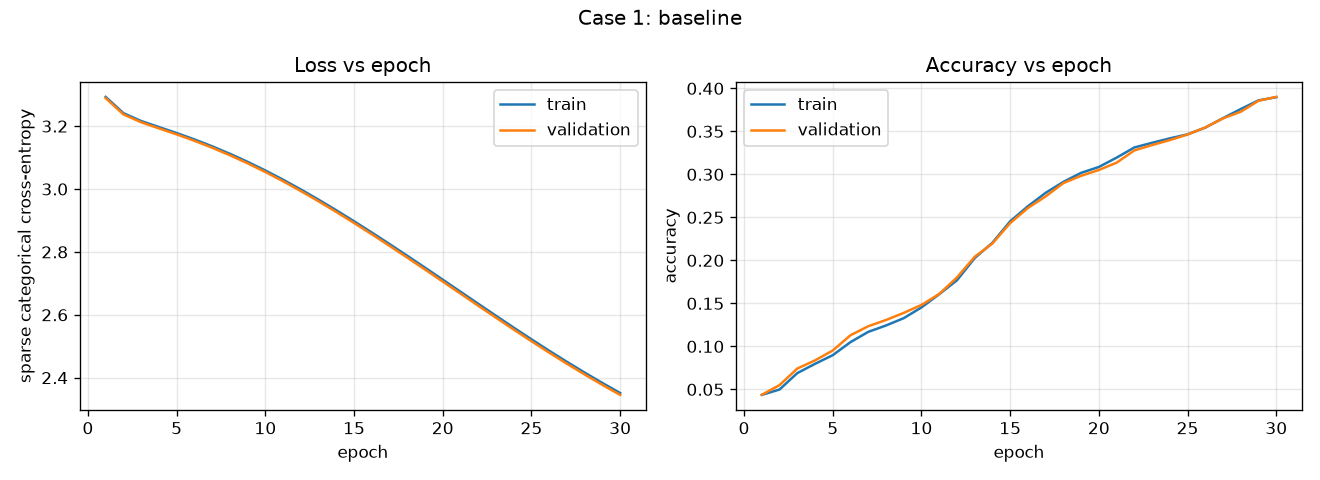
\includegraphics[width=0.95\linewidth]{exp2_case1.png}
\caption{Baseline (the selected case). Training and validation curves lie almost
on top of each other and are still climbing at epoch 30. This is the signature
of underfitting.}
\end{figure}

\begin{figure}[H]
\centering
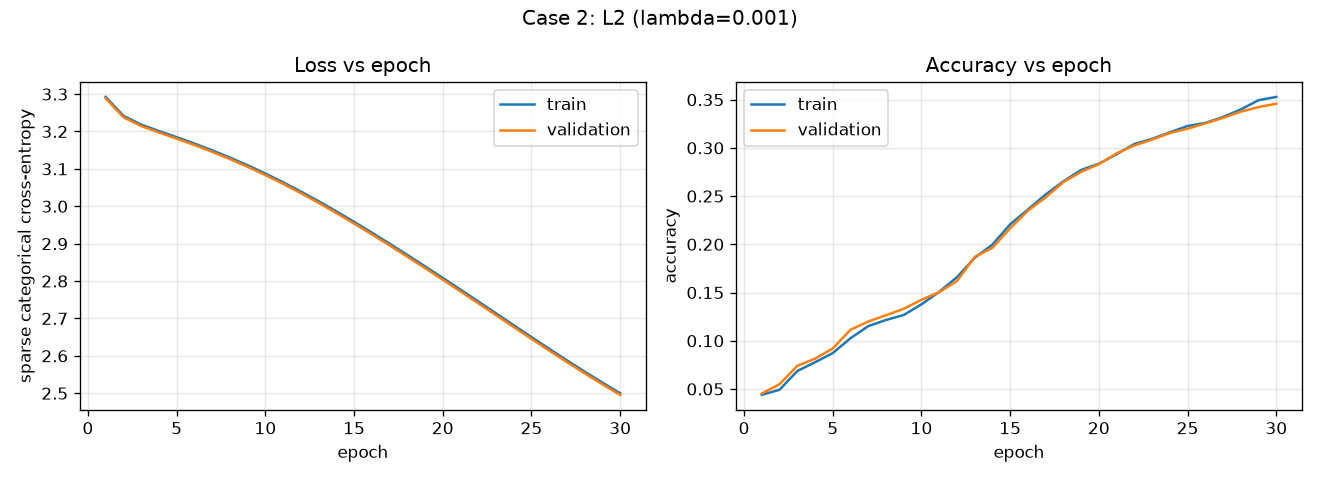
\includegraphics[width=0.95\linewidth]{exp2_case2.png}
\caption{$L_2$ regularization. Same shape as the baseline but slightly worse,
and the final weight norm is smaller ($13.46$ against $15.84$).}
\end{figure}

\begin{figure}[H]
\centering
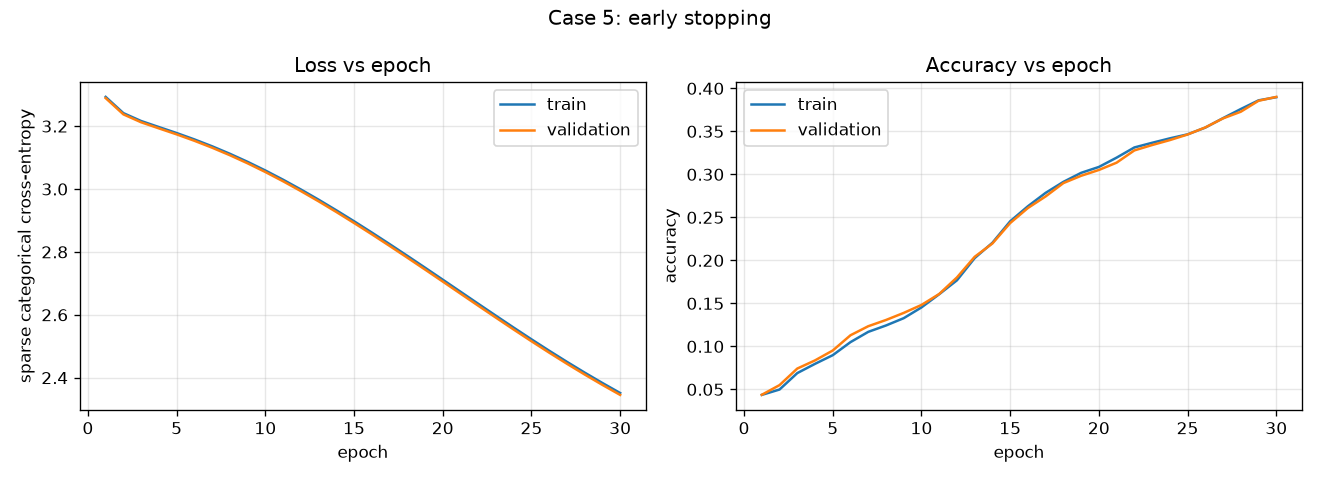
\includegraphics[width=0.95\linewidth]{exp2_case5.png}
\caption{Early stopping. Validation loss decreases every single epoch, so the
patience counter never reaches 5, the run goes the full 30 epochs, and zero
epochs are saved.}
\end{figure}

\begin{figure}[H]
\centering
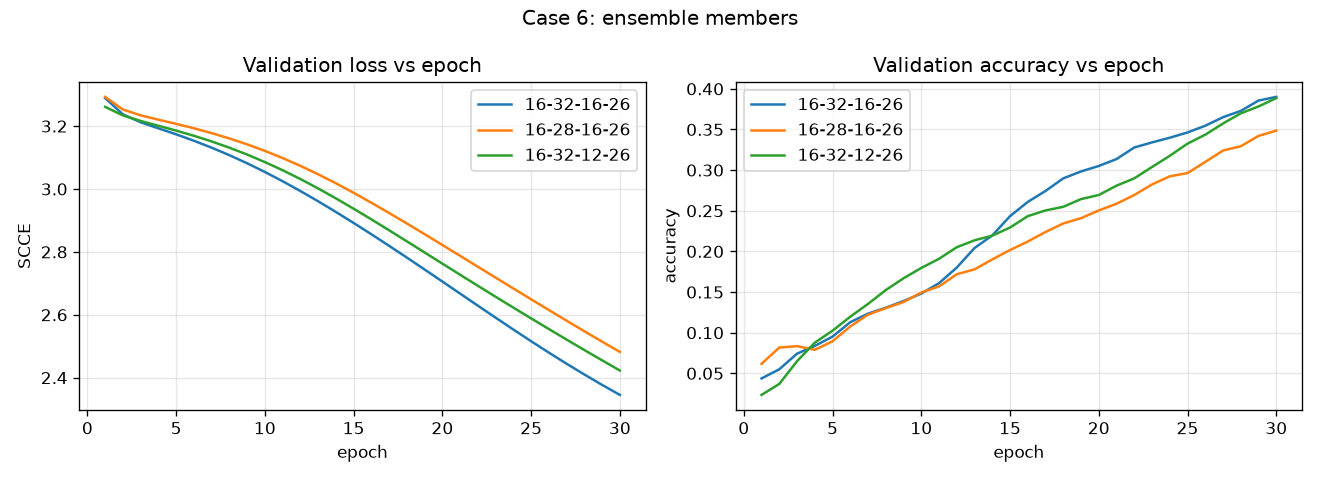
\includegraphics[width=0.95\linewidth]{exp2_case6.png}
\caption{Ensemble members. Three individually mediocre networks whose averaged
prediction beats all of them.}
\end{figure}

\begin{figure}[H]
\centering
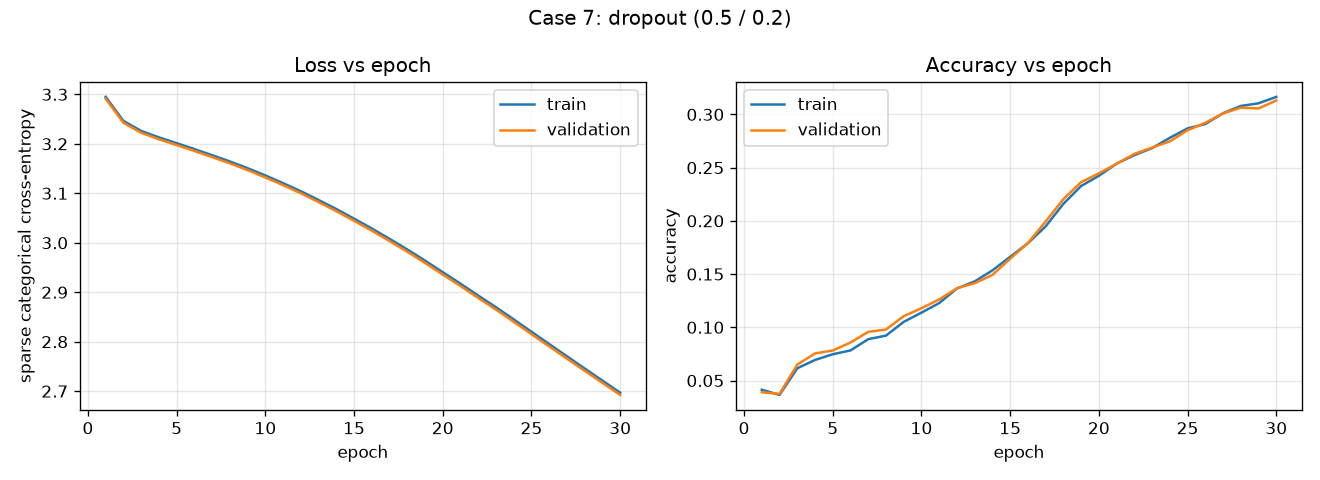
\includegraphics[width=0.95\linewidth]{exp2_case7.png}
\caption{Dropout. The most heavily regularised case, the smallest weight norm
($12.85$), and the lowest accuracy. Dropout removed capacity the model still
needed.}
\end{figure}

\begin{table}[H]
\centering
\begin{tabular}{lccc}
\toprule
Ensemble member & Test accuracy & Test loss & $\|W\|_2$ \\
\midrule
$16\text{-}32\text{-}16\text{-}26$ & 0.3788 & 2.3668 & 15.84 \\
$16\text{-}28\text{-}16\text{-}26$ & 0.3376 & 2.4988 & 14.76 \\
$16\text{-}32\text{-}12\text{-}26$ & 0.3886 & 2.4322 & 14.94 \\
\midrule
average of the three               & \textbf{0.4540} & 2.4110 & n/a \\
\bottomrule
\end{tabular}
\caption{Case 6 broken down. The average is 6.5 points above the best single
member.}
\end{table}

Early stopping details: best epoch $= 30$, stopping epoch $= 30$, epochs saved
$= 0$.

\section{Observation}

\begin{itemize}
\item \textbf{Every model in this experiment is underfitting.} In all seven
      cases the training and validation curves are almost identical and both are
      still rising at epoch 30. There is no generalisation gap to close. With
      the fixed learning rate of $0.001$, 30 epochs, and sigmoid activations,
      the network reaches only about $38\%$ accuracy on a task where a
      well-tuned MLP reaches roughly $90\%$. It has clearly learned something
      real (uniform guessing is under $4\%$), it just has not finished.
\item \textbf{So the pure regularizers hurt, exactly as theory predicts.}
      \begin{itemize}
      \item $L_2$ (Case 2) drops accuracy from $0.379$ to $0.341$. It spent
            gradient budget shrinking weights instead of fitting the data, and
            the weight norm duly fell to $13.46$.
      \item Dropout (Case 7) is worse still, $0.307$, with the smallest norm of
            all, $12.85$. Zeroing half the first hidden layer every step, in a
            network that is already too weak, just makes training slower.
      \end{itemize}
      Both techniques are doing their job correctly. Their job is simply not
      what this underfitting model needs.
\item \textbf{The near-neutral cases behave as expected.} Input noise (Case 3)
      is tiny relative to standardized features, so it changes almost nothing:
      accuracy $0.381$, norm $15.80$, both within noise of the baseline. Early
      stopping (Case 5) is mathematically identical to the baseline here because
      validation loss never stops improving, so it never triggers; best epoch,
      stopping epoch and epochs saved confirm this.
\item \textbf{Label noise (Case 4) did not hurt, and slightly helped.}
      Flipping $10\%$ of training labels raised test accuracy a little, to
      $0.396$. When a model is underfitting, the noisy labels act like a mild
      randomisation that keeps the optimiser moving, similar in spirit to
      adding jitter. On an overfitting model the same corruption would clearly
      lower accuracy.
\item \textbf{The ensemble is the one clear win: $0.454$, about $7.5$ points
      above the baseline.} The three members make different errors because they
      have different architectures and different random initialisations.
      Averaging their probabilities cancels the errors that disagree and keeps
      the predictions they agree on. This works even though each member is
      individually weak, which is the key lesson: ensembling reduces the
      variance part of the error and does not require any single model to be
      good. Its combined weight norm is large ($26.30$) only because it is
      literally three networks.
\item \textbf{Reading the weight-norm column.} It lines up neatly with how much
      each method restrains the function: dropout $12.85 <$ $L_2$ $13.46 <$
      label noise $15.14 <$ input noise $15.80 \approx$ baseline $15.84 <$
      ensemble $26.30$. Smaller is not better here, because smaller came at the
      cost of fitting.
\end{itemize}

\section{Conclusion}

The table tells a consistent story once you notice that every model is
underfitting. Regularizers that work by shrinking the model (L2, dropout)
lowered both the weight norm and the accuracy, because they removed capacity a
still-learning network needed. Regularizers that barely perturb the setup
(small input noise, early stopping that never triggers) left the baseline
essentially unchanged. Mild label noise slightly helped, for the same reason
regularization hurt: the model had room to spare. The only technique that
improved generalisation was the ensemble, which raised test accuracy from
$37.9\%$ to $45.4\%$ by averaging away the independent mistakes of three weak
networks.

The broader lesson is about diagnosis before treatment. Regularization is the
right tool when training accuracy is high and validation accuracy lags behind.
When both are low and still rising, as here, the fix is more capacity, more
epochs, a larger learning rate, or better activations, and adding regularization
on top only slows the model down. Ensembling is the exception: because it
attacks variance rather than capacity, it can help whether the base models are
overfitting or underfitting.

%%%%%%%%%%%%%%%%%%%%%%%%%%%%%%%%%%%%%%%%%%%%%%%%%%%%%%%

\end{document}
